% Options for packages loaded elsewhere
\PassOptionsToPackage{unicode}{hyperref}
\PassOptionsToPackage{hyphens}{url}
%
\documentclass[
]{article}
\usepackage{lmodern}
\usepackage{amsmath}
\usepackage{ifxetex,ifluatex}
\ifnum 0\ifxetex 1\fi\ifluatex 1\fi=0 % if pdftex
  \usepackage[T1]{fontenc}
  \usepackage[utf8]{inputenc}
  \usepackage{textcomp} % provide euro and other symbols
  \usepackage{amssymb}
\else % if luatex or xetex
  \usepackage{unicode-math}
  \defaultfontfeatures{Scale=MatchLowercase}
  \defaultfontfeatures[\rmfamily]{Ligatures=TeX,Scale=1}
\fi
% Use upquote if available, for straight quotes in verbatim environments
\IfFileExists{upquote.sty}{\usepackage{upquote}}{}
\IfFileExists{microtype.sty}{% use microtype if available
  \usepackage[]{microtype}
  \UseMicrotypeSet[protrusion]{basicmath} % disable protrusion for tt fonts
}{}
\makeatletter
\@ifundefined{KOMAClassName}{% if non-KOMA class
  \IfFileExists{parskip.sty}{%
    \usepackage{parskip}
  }{% else
    \setlength{\parindent}{0pt}
    \setlength{\parskip}{6pt plus 2pt minus 1pt}}
}{% if KOMA class
  \KOMAoptions{parskip=half}}
\makeatother
\usepackage{xcolor}
\IfFileExists{xurl.sty}{\usepackage{xurl}}{} % add URL line breaks if available
\IfFileExists{bookmark.sty}{\usepackage{bookmark}}{\usepackage{hyperref}}
\hypersetup{
  pdftitle={Distribuição Normal},
  pdfauthor={Prof.~André Luiz Cunha},
  hidelinks,
  pdfcreator={LaTeX via pandoc}}
\urlstyle{same} % disable monospaced font for URLs
\usepackage[margin=1in]{geometry}
\usepackage{color}
\usepackage{fancyvrb}
\newcommand{\VerbBar}{|}
\newcommand{\VERB}{\Verb[commandchars=\\\{\}]}
\DefineVerbatimEnvironment{Highlighting}{Verbatim}{commandchars=\\\{\}}
% Add ',fontsize=\small' for more characters per line
\usepackage{framed}
\definecolor{shadecolor}{RGB}{248,248,248}
\newenvironment{Shaded}{\begin{snugshade}}{\end{snugshade}}
\newcommand{\AlertTok}[1]{\textcolor[rgb]{0.94,0.16,0.16}{#1}}
\newcommand{\AnnotationTok}[1]{\textcolor[rgb]{0.56,0.35,0.01}{\textbf{\textit{#1}}}}
\newcommand{\AttributeTok}[1]{\textcolor[rgb]{0.77,0.63,0.00}{#1}}
\newcommand{\BaseNTok}[1]{\textcolor[rgb]{0.00,0.00,0.81}{#1}}
\newcommand{\BuiltInTok}[1]{#1}
\newcommand{\CharTok}[1]{\textcolor[rgb]{0.31,0.60,0.02}{#1}}
\newcommand{\CommentTok}[1]{\textcolor[rgb]{0.56,0.35,0.01}{\textit{#1}}}
\newcommand{\CommentVarTok}[1]{\textcolor[rgb]{0.56,0.35,0.01}{\textbf{\textit{#1}}}}
\newcommand{\ConstantTok}[1]{\textcolor[rgb]{0.00,0.00,0.00}{#1}}
\newcommand{\ControlFlowTok}[1]{\textcolor[rgb]{0.13,0.29,0.53}{\textbf{#1}}}
\newcommand{\DataTypeTok}[1]{\textcolor[rgb]{0.13,0.29,0.53}{#1}}
\newcommand{\DecValTok}[1]{\textcolor[rgb]{0.00,0.00,0.81}{#1}}
\newcommand{\DocumentationTok}[1]{\textcolor[rgb]{0.56,0.35,0.01}{\textbf{\textit{#1}}}}
\newcommand{\ErrorTok}[1]{\textcolor[rgb]{0.64,0.00,0.00}{\textbf{#1}}}
\newcommand{\ExtensionTok}[1]{#1}
\newcommand{\FloatTok}[1]{\textcolor[rgb]{0.00,0.00,0.81}{#1}}
\newcommand{\FunctionTok}[1]{\textcolor[rgb]{0.00,0.00,0.00}{#1}}
\newcommand{\ImportTok}[1]{#1}
\newcommand{\InformationTok}[1]{\textcolor[rgb]{0.56,0.35,0.01}{\textbf{\textit{#1}}}}
\newcommand{\KeywordTok}[1]{\textcolor[rgb]{0.13,0.29,0.53}{\textbf{#1}}}
\newcommand{\NormalTok}[1]{#1}
\newcommand{\OperatorTok}[1]{\textcolor[rgb]{0.81,0.36,0.00}{\textbf{#1}}}
\newcommand{\OtherTok}[1]{\textcolor[rgb]{0.56,0.35,0.01}{#1}}
\newcommand{\PreprocessorTok}[1]{\textcolor[rgb]{0.56,0.35,0.01}{\textit{#1}}}
\newcommand{\RegionMarkerTok}[1]{#1}
\newcommand{\SpecialCharTok}[1]{\textcolor[rgb]{0.00,0.00,0.00}{#1}}
\newcommand{\SpecialStringTok}[1]{\textcolor[rgb]{0.31,0.60,0.02}{#1}}
\newcommand{\StringTok}[1]{\textcolor[rgb]{0.31,0.60,0.02}{#1}}
\newcommand{\VariableTok}[1]{\textcolor[rgb]{0.00,0.00,0.00}{#1}}
\newcommand{\VerbatimStringTok}[1]{\textcolor[rgb]{0.31,0.60,0.02}{#1}}
\newcommand{\WarningTok}[1]{\textcolor[rgb]{0.56,0.35,0.01}{\textbf{\textit{#1}}}}
\usepackage{graphicx}
\makeatletter
\def\maxwidth{\ifdim\Gin@nat@width>\linewidth\linewidth\else\Gin@nat@width\fi}
\def\maxheight{\ifdim\Gin@nat@height>\textheight\textheight\else\Gin@nat@height\fi}
\makeatother
% Scale images if necessary, so that they will not overflow the page
% margins by default, and it is still possible to overwrite the defaults
% using explicit options in \includegraphics[width, height, ...]{}
\setkeys{Gin}{width=\maxwidth,height=\maxheight,keepaspectratio}
% Set default figure placement to htbp
\makeatletter
\def\fps@figure{htbp}
\makeatother
\setlength{\emergencystretch}{3em} % prevent overfull lines
\providecommand{\tightlist}{%
  \setlength{\itemsep}{0pt}\setlength{\parskip}{0pt}}
\setcounter{secnumdepth}{5}
\usepackage{caption}
\usepackage[portuguese]{babel}
\ifluatex
  \usepackage{selnolig}  % disable illegal ligatures
\fi

\title{Distribuição Normal}
\usepackage{etoolbox}
\makeatletter
\providecommand{\subtitle}[1]{% add subtitle to \maketitle
  \apptocmd{\@title}{\par {\large #1 \par}}{}{}
}
\makeatother
\subtitle{Aula 2}
\author{Prof.~André Luiz Cunha}
\date{21/05/2021}

\begin{document}
\maketitle

\hypertarget{transformauxe7uxe3o-de-escala}{%
\section{Transformação de escala}\label{transformauxe7uxe3o-de-escala}}

Um passo importante de qualquer análise de dados é a uniformização do
intervalo de dados, de modo que todas as variáveis do banco de dados
tenham o mesmo intervalo de variação.

Seja o exemplo do conjunto de dados aleatório abaixo, são apresentados
dois tipos de transformação encontrados na literatura.

\begin{Shaded}
\begin{Highlighting}[]
\CommentTok{\# Conjunto de valores aleatórios com média 50 e desvio 15.}
\NormalTok{(x }\OtherTok{\textless{}{-}} \FunctionTok{rnorm}\NormalTok{(}\DecValTok{100}\NormalTok{, }\DecValTok{50}\NormalTok{, }\DecValTok{15}\NormalTok{))}
\end{Highlighting}
\end{Shaded}

\begin{verbatim}
##   [1] 67.38209 44.36467 53.80939 41.33888 51.60008 54.31530 61.89694 45.33601
##   [9] 60.76003 65.07051 40.53391 35.18354 55.74108 54.07982 36.79692 55.87327
##  [17] 32.93785 37.29865 46.96603 37.63343 53.79591 37.12693 52.32424 43.21072
##  [25] 53.20274 27.54581 52.22474 38.83846 57.11614 68.78142 54.43861 49.09645
##  [33] 19.13876 59.21151 49.28278 50.96855 76.42924 62.61803 65.64291 38.92497
##  [41] 63.61846 53.22992 48.17272 41.52407 42.59956 26.12273 37.13655 36.17765
##  [49] 27.79757 48.58399 19.93381 41.39033 22.66142 65.34623 74.32932 64.87410
##  [57] 61.96386 70.37860 34.95970 49.56880 63.71918 37.05237 60.04204 62.99392
##  [65] 63.36854 26.33910 60.65801 43.19757 44.96063 45.94747 29.23396 42.26117
##  [73] 57.44031 52.76061 69.90471 29.75177 46.80179 60.51939 74.13881 43.52736
##  [81] 80.58713 56.49009 59.40942 44.13878 35.62000 37.41026 44.42762 62.02210
##  [89] 50.20614 27.40463 36.73793 40.95965 35.47438 38.82704 31.44681 27.83082
##  [97] 43.80613 19.71721 24.16069 53.54825
\end{verbatim}

\begin{Shaded}
\begin{Highlighting}[]
\FunctionTok{summary}\NormalTok{(x)}
\end{Highlighting}
\end{Shaded}

\begin{verbatim}
##    Min. 1st Qu.  Median    Mean 3rd Qu.    Max. 
##   19.14   37.26   47.57   47.84   59.26   80.59
\end{verbatim}

\hypertarget{normalizauxe7uxe3o-01}{%
\subsection{Normalização {[}0,1{]}}\label{normalizauxe7uxe3o-01}}

A normalização transforma os dados no intervalo entre 0 e 1.

\begin{Shaded}
\begin{Highlighting}[]
\NormalTok{x\_norm }\OtherTok{\textless{}{-}}\NormalTok{ (x }\SpecialCharTok{{-}} \FunctionTok{min}\NormalTok{(x)) }\SpecialCharTok{/}\NormalTok{ (}\FunctionTok{max}\NormalTok{(x) }\SpecialCharTok{{-}} \FunctionTok{min}\NormalTok{(x))}
\FunctionTok{summary}\NormalTok{(x\_norm)}
\end{Highlighting}
\end{Shaded}

\begin{verbatim}
##    Min. 1st Qu.  Median    Mean 3rd Qu.    Max. 
##  0.0000  0.2949  0.4627  0.4671  0.6529  1.0000
\end{verbatim}

\hypertarget{padronizar--33}{%
\subsection{Padronizar {[}-3,3{]}}\label{padronizar--33}}

A padronização dos dados nada mais é do que a transformação para a
escala da curva normal padrão (z-padrão). Vide Figura 1 a tabela
z-padrão.

\begin{Shaded}
\begin{Highlighting}[]
\NormalTok{x\_pad }\OtherTok{\textless{}{-}}\NormalTok{ (x }\SpecialCharTok{{-}} \FunctionTok{mean}\NormalTok{(x)) }\SpecialCharTok{/} \FunctionTok{sd}\NormalTok{(x)}
\FunctionTok{summary}\NormalTok{(x\_pad)}
\end{Highlighting}
\end{Shaded}

\begin{verbatim}
##     Min.  1st Qu.   Median     Mean  3rd Qu.     Max. 
## -2.04903 -0.75548 -0.01936  0.00000  0.81531  2.33780
\end{verbatim}

\begin{figure}

{\centering 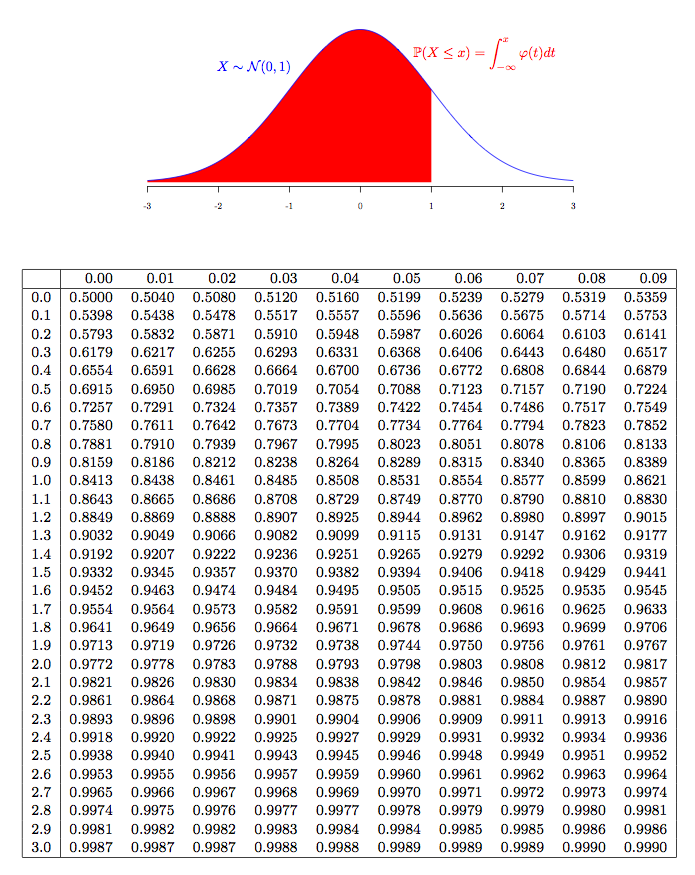
\includegraphics[width=0.6\linewidth]{normal-table} 

}

\caption{Tabela z-padrão}\label{fig:ztable}
\end{figure}

\begin{Shaded}
\begin{Highlighting}[]
\DocumentationTok{\#\# OLHANDO A TABELA}
\CommentTok{\#z = 1,0 {-}{-}{-}{-}\textgreater{} p(z) = 0,1587}
\DecValTok{1} \SpecialCharTok{{-}} \DecValTok{2} \SpecialCharTok{*} \FloatTok{0.1587}
\end{Highlighting}
\end{Shaded}

\begin{verbatim}
## [1] 0.6826
\end{verbatim}

\begin{Shaded}
\begin{Highlighting}[]
\CommentTok{\#z = 2,0 {-}{-}{-}{-}\textgreater{} p(z) = 0,0228}
\DecValTok{1} \SpecialCharTok{{-}} \DecValTok{2} \SpecialCharTok{*} \FloatTok{0.0228}
\end{Highlighting}
\end{Shaded}

\begin{verbatim}
## [1] 0.9544
\end{verbatim}

\begin{Shaded}
\begin{Highlighting}[]
\CommentTok{\# p(z) = 95\% {-}{-}{-}{-}{-}\textgreater{} z(p = 0,025) = ?}
\FloatTok{1.96}
\end{Highlighting}
\end{Shaded}

\begin{verbatim}
## [1] 1.96
\end{verbatim}

\begin{Shaded}
\begin{Highlighting}[]
\CommentTok{\# p(z) = 99\% {-}{-}{-}{-}{-}\textgreater{} z =??}
\FloatTok{2.575}
\end{Highlighting}
\end{Shaded}

\begin{verbatim}
## [1] 2.575
\end{verbatim}

\hypertarget{funuxe7uxf5es-do-r}{%
\section{Funções do R}\label{funuxe7uxf5es-do-r}}

\hypertarget{nuxfameros-aleatuxf3rios}{%
\subsection{Números aleatórios}\label{nuxfameros-aleatuxf3rios}}

\begin{Shaded}
\begin{Highlighting}[]
\DocumentationTok{\#\# Uniformemente distribuídos}
\end{Highlighting}
\end{Shaded}

Função: \texttt{runif(n,\ min,\ max)}

\begin{Shaded}
\begin{Highlighting}[]
\FunctionTok{runif}\NormalTok{(}\DecValTok{10}\NormalTok{)}
\end{Highlighting}
\end{Shaded}

\begin{verbatim}
##  [1] 0.2921710 0.1243811 0.7045777 0.9484180 0.5995654 0.8572610 0.9077824
##  [8] 0.5266294 0.4437137 0.8350196
\end{verbatim}

\begin{Shaded}
\begin{Highlighting}[]
\FunctionTok{runif}\NormalTok{(}\DecValTok{10}\NormalTok{, }\DecValTok{100}\NormalTok{, }\DecValTok{150}\NormalTok{)}
\end{Highlighting}
\end{Shaded}

\begin{verbatim}
##  [1] 137.2926 117.7441 118.1983 144.7208 142.3846 146.1939 135.9226 116.5154
##  [9] 117.0558 133.1327
\end{verbatim}

\begin{Shaded}
\begin{Highlighting}[]
\FunctionTok{hist}\NormalTok{(}\FunctionTok{runif}\NormalTok{(}\DecValTok{10000}\NormalTok{))}
\end{Highlighting}
\end{Shaded}

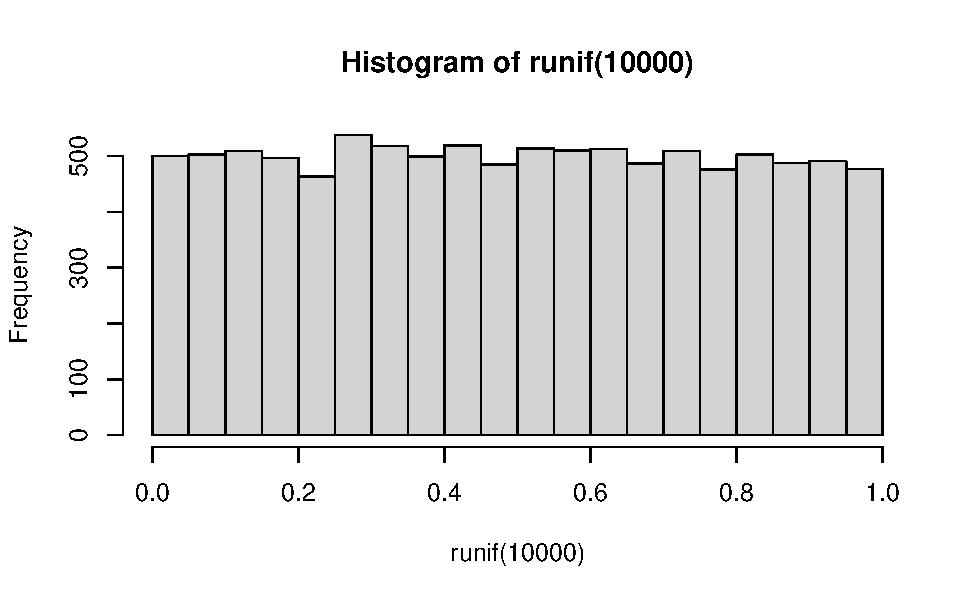
\includegraphics{DistNormal_files/figure-latex/unnamed-chunk-6-1.pdf}

\begin{Shaded}
\begin{Highlighting}[]
\DocumentationTok{\#\# Normalmente distribuídos}
\end{Highlighting}
\end{Shaded}

Função: \texttt{rnorm(n,\ mean,\ sd)}

\begin{Shaded}
\begin{Highlighting}[]
\FunctionTok{rnorm}\NormalTok{(}\DecValTok{10}\NormalTok{)}
\end{Highlighting}
\end{Shaded}

\begin{verbatim}
##  [1]  0.01682654  0.51782051 -0.52881088  0.31302410 -0.72271552  0.38712121
##  [7]  0.40100879  0.87852581  1.70679692 -2.34912372
\end{verbatim}

\begin{Shaded}
\begin{Highlighting}[]
\FunctionTok{rnorm}\NormalTok{(}\DecValTok{10}\NormalTok{, }\DecValTok{100}\NormalTok{, }\DecValTok{15}\NormalTok{)}
\end{Highlighting}
\end{Shaded}

\begin{verbatim}
##  [1] 103.13431  94.11965  92.94349 104.12939  88.03196  95.35177 104.54607
##  [8] 102.47912 103.32911  85.33530
\end{verbatim}

\begin{Shaded}
\begin{Highlighting}[]
\FunctionTok{hist}\NormalTok{(}\FunctionTok{rnorm}\NormalTok{(}\DecValTok{10000}\NormalTok{), }\AttributeTok{breaks =} \FunctionTok{seq}\NormalTok{(}\SpecialCharTok{{-}}\DecValTok{5}\NormalTok{,}\DecValTok{5}\NormalTok{,.}\DecValTok{1}\NormalTok{),}
     \AttributeTok{freq =} \ConstantTok{FALSE}\NormalTok{)}
\end{Highlighting}
\end{Shaded}

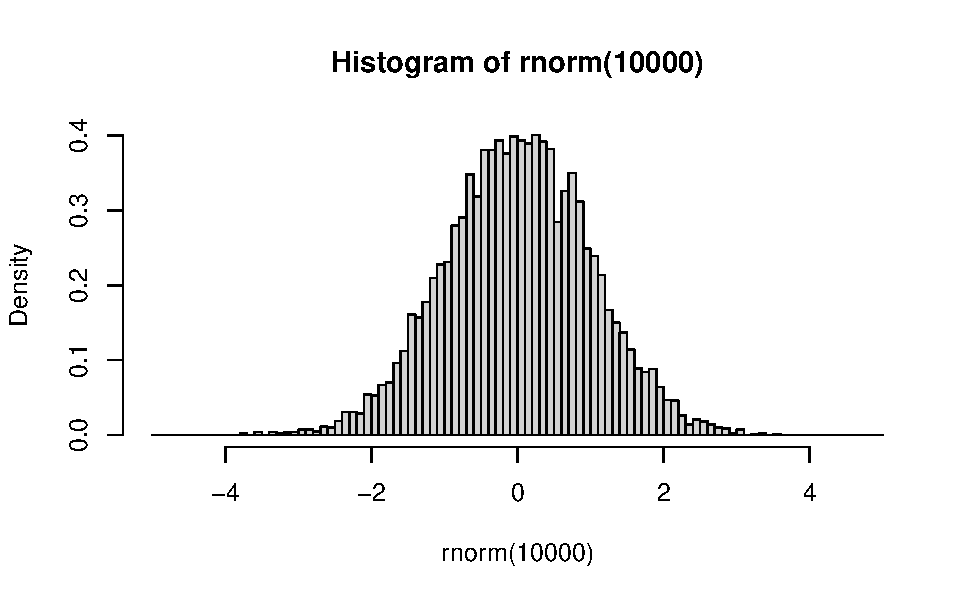
\includegraphics{DistNormal_files/figure-latex/unnamed-chunk-7-1.pdf}

\hypertarget{distribuiuxe7uxe3o-normal}{%
\subsection{Distribuição Normal}\label{distribuiuxe7uxe3o-normal}}

Encontrando o valor z-padrão com a função
\texttt{qnorm(area\ da\ curva,\ mean=0,\ sd=1)}

\begin{itemize}
\tightlist
\item
  Unicaudal a esquerda: \texttt{z\_alpha\ =\ qnorm(alpha)}
\item
  Unicaudal a direita: \texttt{z\_alpha\ =\ qnorm(1\ -\ alpha)}
\item
  Bicaudal: \texttt{z\_alpha/2\ =\ qnorm(1\ -\ alpha/2)}
\end{itemize}

\begin{Shaded}
\begin{Highlighting}[]
\FunctionTok{qnorm}\NormalTok{(.}\DecValTok{90}\NormalTok{)}
\end{Highlighting}
\end{Shaded}

\begin{verbatim}
## [1] 1.281552
\end{verbatim}

\begin{Shaded}
\begin{Highlighting}[]
\FunctionTok{qnorm}\NormalTok{(.}\DecValTok{5}\NormalTok{)}
\end{Highlighting}
\end{Shaded}

\begin{verbatim}
## [1] 0
\end{verbatim}

Encontrando o p-valor com a função
\texttt{pnorm(valor\ z,\ mean=0,\ sd=1)}

\begin{itemize}
\tightlist
\item
  Unicaudal a esquerda: \texttt{p-value\ =\ pnorm(z,\ lower.tail=TRUE)}
\item
  Unicaudal a direita: \texttt{p-value\ =\ pnorm(z,\ lower.tail=FALSE)}
\item
  Bicaudal: \texttt{p-value\ =\ 2\ *\ pnorm(abs(z),\ lower.tail=FALSE)}
\end{itemize}

\begin{Shaded}
\begin{Highlighting}[]
\FunctionTok{pnorm}\NormalTok{(}\FloatTok{1.96}\NormalTok{)}
\end{Highlighting}
\end{Shaded}

\begin{verbatim}
## [1] 0.9750021
\end{verbatim}

\begin{Shaded}
\begin{Highlighting}[]
\FunctionTok{pnorm}\NormalTok{(}\FloatTok{1.96}\NormalTok{, }\AttributeTok{lower.tail =} \ConstantTok{FALSE}\NormalTok{)}
\end{Highlighting}
\end{Shaded}

\begin{verbatim}
## [1] 0.0249979
\end{verbatim}

\begin{Shaded}
\begin{Highlighting}[]
\FunctionTok{pnorm}\NormalTok{(}\DecValTok{0}\NormalTok{)}
\end{Highlighting}
\end{Shaded}

\begin{verbatim}
## [1] 0.5
\end{verbatim}

Encontrando a densidade do valor com a função
\texttt{dnorm(valor\ z,\ mean=0,\ sd=1)}

\begin{Shaded}
\begin{Highlighting}[]
\FunctionTok{dnorm}\NormalTok{(}\FloatTok{1.96}\NormalTok{)}
\end{Highlighting}
\end{Shaded}

\begin{verbatim}
## [1] 0.05844094
\end{verbatim}

\begin{Shaded}
\begin{Highlighting}[]
\FunctionTok{dnorm}\NormalTok{(}\SpecialCharTok{{-}}\FloatTok{1.96}\NormalTok{)}
\end{Highlighting}
\end{Shaded}

\begin{verbatim}
## [1] 0.05844094
\end{verbatim}

\begin{Shaded}
\begin{Highlighting}[]
\FunctionTok{dnorm}\NormalTok{(}\DecValTok{0}\NormalTok{)}
\end{Highlighting}
\end{Shaded}

\begin{verbatim}
## [1] 0.3989423
\end{verbatim}

\textbf{EXEMPLO 1}

\begin{Shaded}
\begin{Highlighting}[]
\DocumentationTok{\#\# P(z \textgreater{} 1,65)}
\FunctionTok{pnorm}\NormalTok{(}\FloatTok{1.65}\NormalTok{, }\AttributeTok{lower.tail =} \ConstantTok{FALSE}\NormalTok{)}
\end{Highlighting}
\end{Shaded}

\begin{verbatim}
## [1] 0.04947147
\end{verbatim}

\begin{Shaded}
\begin{Highlighting}[]
\DocumentationTok{\#\# P(z \textless{} 1,65)}
\FunctionTok{pnorm}\NormalTok{(}\FloatTok{1.65}\NormalTok{)}
\end{Highlighting}
\end{Shaded}

\begin{verbatim}
## [1] 0.9505285
\end{verbatim}

\begin{Shaded}
\begin{Highlighting}[]
\DocumentationTok{\#\# P(1,40 \textless{} z \textless{} 1,70)}
\FunctionTok{pnorm}\NormalTok{(}\FloatTok{1.7}\NormalTok{) }\SpecialCharTok{{-}} \FunctionTok{pnorm}\NormalTok{(}\FloatTok{1.4}\NormalTok{)}
\end{Highlighting}
\end{Shaded}

\begin{verbatim}
## [1] 0.0361912
\end{verbatim}

\textbf{EXEMPLO 2}

\begin{Shaded}
\begin{Highlighting}[]
\NormalTok{x }\OtherTok{=} \FunctionTok{c}\NormalTok{(}\DecValTok{58}\NormalTok{,}\DecValTok{78}\NormalTok{,}\DecValTok{84}\NormalTok{,}\DecValTok{90}\NormalTok{,}\DecValTok{97}\NormalTok{,}\DecValTok{70}\NormalTok{,}
      \DecValTok{90}\NormalTok{,}\DecValTok{86}\NormalTok{,}\DecValTok{82}\NormalTok{,}\DecValTok{59}\NormalTok{,}\DecValTok{90}\NormalTok{,}\DecValTok{70}\NormalTok{,}
      \DecValTok{74}\NormalTok{,}\DecValTok{83}\NormalTok{,}\DecValTok{90}\NormalTok{,}\DecValTok{75}\NormalTok{,}\DecValTok{88}\NormalTok{,}\DecValTok{84}\NormalTok{,}
      \DecValTok{68}\NormalTok{,}\DecValTok{96}\NormalTok{,}\DecValTok{70}\NormalTok{,}\DecValTok{94}\NormalTok{,}\DecValTok{70}\NormalTok{,}\DecValTok{110}\NormalTok{,}
      \DecValTok{67}\NormalTok{,}\DecValTok{68}\NormalTok{,}\DecValTok{75}\NormalTok{,}\DecValTok{80}\NormalTok{,}\DecValTok{68}\NormalTok{,}\DecValTok{82}\NormalTok{,}
      \DecValTok{104}\NormalTok{,}\DecValTok{92}\NormalTok{,}\DecValTok{112}\NormalTok{,}\DecValTok{84}\NormalTok{,}\DecValTok{98}\NormalTok{,}\DecValTok{80}\NormalTok{)}


\DocumentationTok{\#\# Análise descritiva}
\FunctionTok{summary}\NormalTok{(x)}
\end{Highlighting}
\end{Shaded}

\begin{verbatim}
##    Min. 1st Qu.  Median    Mean 3rd Qu.    Max. 
##   58.00   70.00   82.50   82.39   90.00  112.00
\end{verbatim}

\begin{Shaded}
\begin{Highlighting}[]
\NormalTok{hdados }\OtherTok{\textless{}{-}} \FunctionTok{hist}\NormalTok{(x, }
               \AttributeTok{breaks =} \FunctionTok{seq}\NormalTok{(}\DecValTok{40}\NormalTok{,}\DecValTok{140}\NormalTok{,}\DecValTok{10}\NormalTok{))}
\end{Highlighting}
\end{Shaded}

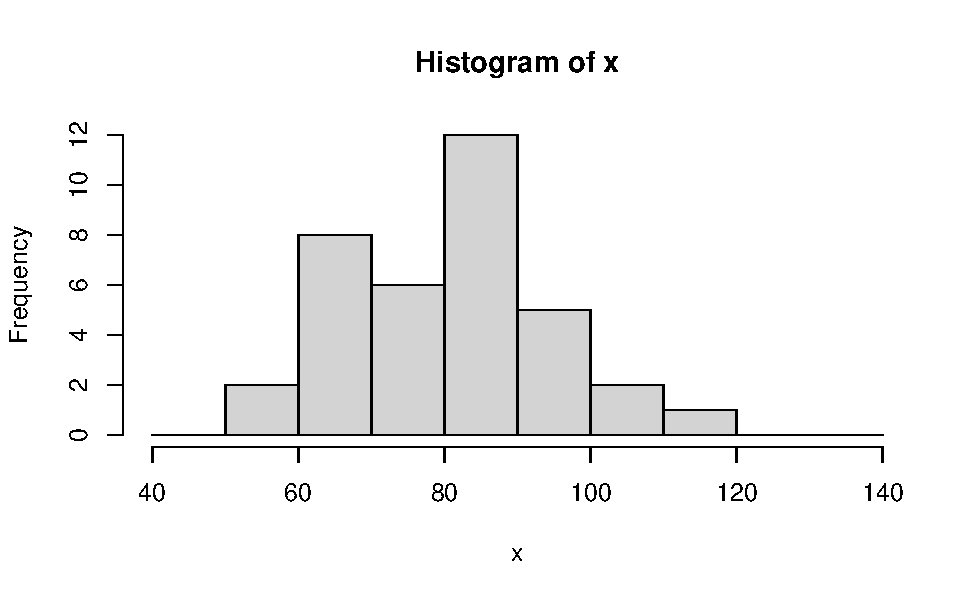
\includegraphics{DistNormal_files/figure-latex/unnamed-chunk-12-1.pdf}

\begin{Shaded}
\begin{Highlighting}[]
\NormalTok{hdados}\SpecialCharTok{$}\NormalTok{breaks}
\end{Highlighting}
\end{Shaded}

\begin{verbatim}
##  [1]  40  50  60  70  80  90 100 110 120 130 140
\end{verbatim}

\begin{Shaded}
\begin{Highlighting}[]
\NormalTok{hdados}\SpecialCharTok{$}\NormalTok{counts}
\end{Highlighting}
\end{Shaded}

\begin{verbatim}
##  [1]  0  2  8  6 12  5  2  1  0  0
\end{verbatim}

\begin{Shaded}
\begin{Highlighting}[]
\NormalTok{hdados}\SpecialCharTok{$}\NormalTok{density}
\end{Highlighting}
\end{Shaded}

\begin{verbatim}
##  [1] 0.000000000 0.005555556 0.022222222 0.016666667 0.033333333 0.013888889
##  [7] 0.005555556 0.002777778 0.000000000 0.000000000
\end{verbatim}

O parâmetro \texttt{density} traz a razão entre a porcentagem de
elementos e o intervalo de bins, tanto que a soma das porcentagens
\texttt{density} é igual a\\
\texttt{0.1}

\begin{Shaded}
\begin{Highlighting}[]
\CommentTok{\#. }

\FunctionTok{sum}\NormalTok{(hdados}\SpecialCharTok{$}\NormalTok{density)}
\end{Highlighting}
\end{Shaded}

\begin{verbatim}
## [1] 0.1
\end{verbatim}

Ao multiplicar cada densidade pelo intervalo do bin, a porcentagem total
será de 100\%.

\begin{Shaded}
\begin{Highlighting}[]
\FunctionTok{sum}\NormalTok{(hdados}\SpecialCharTok{$}\NormalTok{density) }\SpecialCharTok{*} \DecValTok{10}
\end{Highlighting}
\end{Shaded}

\begin{verbatim}
## [1] 1
\end{verbatim}

\hypertarget{testes-do-r}{%
\section{Testes do R}\label{testes-do-r}}

\begin{Shaded}
\begin{Highlighting}[]
\NormalTok{x\_pad }\OtherTok{\textless{}{-}}\NormalTok{ (x }\SpecialCharTok{{-}} \FunctionTok{mean}\NormalTok{(x))}\SpecialCharTok{/}\FunctionTok{sd}\NormalTok{(x)}
\end{Highlighting}
\end{Shaded}

\hypertarget{qui-quadrado}{%
\subsection{Qui-quadrado}\label{qui-quadrado}}

Teste de aderência de Qui-quadrado é usado para compara distribuições
observadas com distribuições esperadas em dados discretos (histogramas
de frequências).

\begin{Shaded}
\begin{Highlighting}[]
\DocumentationTok{\#\# Densidade dos valores X com a curva normal teórica}
\NormalTok{bin }\OtherTok{\textless{}{-}} \DecValTok{10}
\NormalTok{hist.real }\OtherTok{\textless{}{-}} \FunctionTok{hist}\NormalTok{(x, }\AttributeTok{breaks =} \FunctionTok{seq}\NormalTok{(}\DecValTok{40}\NormalTok{,}\DecValTok{140}\NormalTok{,bin), }\AttributeTok{freq=}\ConstantTok{FALSE}\NormalTok{)}
\FunctionTok{curve}\NormalTok{(}\FunctionTok{dnorm}\NormalTok{(x, }\FunctionTok{mean}\NormalTok{(x), }\FunctionTok{sd}\NormalTok{(x)), }\AttributeTok{col=}\StringTok{\textquotesingle{}darkblue\textquotesingle{}}\NormalTok{, }\AttributeTok{lw=}\DecValTok{2}\NormalTok{, }\AttributeTok{add=}\ConstantTok{TRUE}\NormalTok{)}
\end{Highlighting}
\end{Shaded}

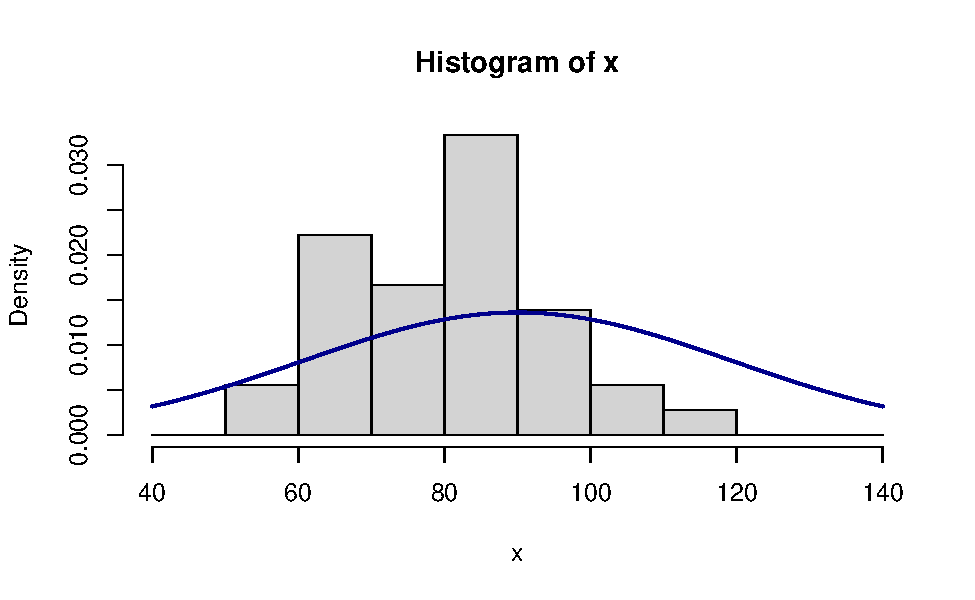
\includegraphics{DistNormal_files/figure-latex/unnamed-chunk-16-1.pdf}

\begin{Shaded}
\begin{Highlighting}[]
\NormalTok{hist.real}\SpecialCharTok{$}\NormalTok{density}
\end{Highlighting}
\end{Shaded}

\begin{verbatim}
##  [1] 0.000000000 0.005555556 0.022222222 0.016666667 0.033333333 0.013888889
##  [7] 0.005555556 0.002777778 0.000000000 0.000000000
\end{verbatim}

\begin{Shaded}
\begin{Highlighting}[]
\NormalTok{hist.real}\SpecialCharTok{$}\NormalTok{counts}
\end{Highlighting}
\end{Shaded}

\begin{verbatim}
##  [1]  0  2  8  6 12  5  2  1  0  0
\end{verbatim}

\begin{Shaded}
\begin{Highlighting}[]
\DocumentationTok{\#\# Frequências das distribuições observadas e esperadas}
\FunctionTok{barplot}\NormalTok{(}\FunctionTok{rbind}\NormalTok{(hist.real}\SpecialCharTok{$}\NormalTok{counts, }\FunctionTok{dnorm}\NormalTok{(hist.real}\SpecialCharTok{$}\NormalTok{mids, }\FunctionTok{mean}\NormalTok{(x), }\FunctionTok{sd}\NormalTok{(x))}\SpecialCharTok{*}\NormalTok{bin}\SpecialCharTok{*}\FunctionTok{length}\NormalTok{(x) ),}
        \AttributeTok{names.arg =}\NormalTok{ hist.real}\SpecialCharTok{$}\NormalTok{mids,}
        \AttributeTok{col =} \FunctionTok{c}\NormalTok{(}\StringTok{"darkblue"}\NormalTok{, }\StringTok{"red"}\NormalTok{),}
        \AttributeTok{beside =} \ConstantTok{TRUE}
\NormalTok{)}
\end{Highlighting}
\end{Shaded}

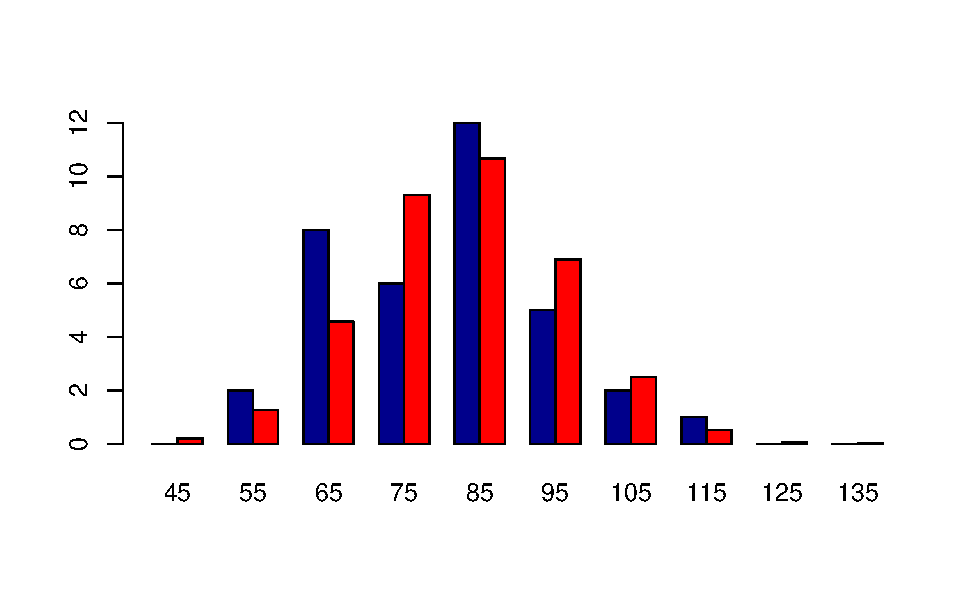
\includegraphics{DistNormal_files/figure-latex/unnamed-chunk-16-2.pdf}

\begin{Shaded}
\begin{Highlighting}[]
\FunctionTok{chisq.test}\NormalTok{(hist.real}\SpecialCharTok{$}\NormalTok{counts, }\CommentTok{\# Frequência observada {-} dados originais}
           \AttributeTok{p =} \FunctionTok{dnorm}\NormalTok{(hist.real}\SpecialCharTok{$}\NormalTok{mids, }\FunctionTok{mean}\NormalTok{(x), }\FunctionTok{sd}\NormalTok{(x))}\SpecialCharTok{*}\NormalTok{bin, }\CommentTok{\# Frequência teórica {-} distribuição normal}
           \AttributeTok{rescale.p =} \ConstantTok{TRUE}\NormalTok{ ) }
\end{Highlighting}
\end{Shaded}

\begin{verbatim}
## Warning in chisq.test(hist.real$counts, p = dnorm(hist.real$mids, mean(x), :
## Chi-squared approximation may be incorrect
\end{verbatim}

\begin{verbatim}
## 
##  Chi-squared test for given probabilities
## 
## data:  hist.real$counts
## X-squared = 5.7035, df = 9, p-value = 0.7692
\end{verbatim}

\hypertarget{kolmogorv-smirnov-ks}{%
\subsection{Kolmogorv-Smirnov (KS)}\label{kolmogorv-smirnov-ks}}

\begin{Shaded}
\begin{Highlighting}[]
\FunctionTok{ks.test}\NormalTok{(x, }\StringTok{"pnorm"}\NormalTok{, }\FunctionTok{mean}\NormalTok{(x), }\FunctionTok{sd}\NormalTok{(x))}
\end{Highlighting}
\end{Shaded}

\begin{verbatim}
## Warning in ks.test(x, "pnorm", mean(x), sd(x)): ties should not be present for
## the Kolmogorov-Smirnov test
\end{verbatim}

\begin{verbatim}
## 
##  One-sample Kolmogorov-Smirnov test
## 
## data:  x
## D = 0.10407, p-value = 0.8304
## alternative hypothesis: two-sided
\end{verbatim}

\begin{Shaded}
\begin{Highlighting}[]
\FunctionTok{ks.test}\NormalTok{(x\_pad, }\StringTok{"pnorm"}\NormalTok{)}
\end{Highlighting}
\end{Shaded}

\begin{verbatim}
## Warning in ks.test(x_pad, "pnorm"): ties should not be present for the
## Kolmogorov-Smirnov test
\end{verbatim}

\begin{verbatim}
## 
##  One-sample Kolmogorov-Smirnov test
## 
## data:  x_pad
## D = 0.10407, p-value = 0.8304
## alternative hypothesis: two-sided
\end{verbatim}

\hypertarget{shapiro-wilk}{%
\subsection{Shapiro-Wilk}\label{shapiro-wilk}}

\begin{Shaded}
\begin{Highlighting}[]
\FunctionTok{shapiro.test}\NormalTok{(x)}
\end{Highlighting}
\end{Shaded}

\begin{verbatim}
## 
##  Shapiro-Wilk normality test
## 
## data:  x
## W = 0.97612, p-value = 0.6139
\end{verbatim}

\end{document}
